\icode{E-MD-CA-L3-261120-001}
如图所示，劲度系数为 \(k\) 的轻弹簧的一端固定在墙上，另一端与置于水平面上质量均为 \(m\) 的物体 \(A\)、\(B\) 接触（\(A\) 与 \(B\) 和弹簧均未连接），弹簧水平且无形变。用水平力 \(F\) 缓慢推动物体 \(B\)，在弹性限度内弹簧长度被压缩了 \(x_0\)，此时物体 \(A\)、\(B\) 静止。已知物体 \(A\) 与水平面间的动摩擦因数为\(\mu\)，物体 \(B\) 与水平面间的摩擦不计。撤去 	\(F\)后，物体 \(A\)、\(B\) 开始向左运动，求分离时弹簧的弹力大小。

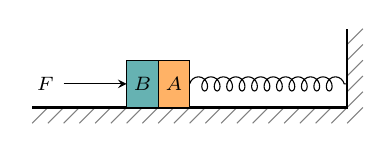
\begin{tikzpicture}[>=stealth,font=\scriptsize]
	\foreach \y in {0,.2,...,.8}
		\draw[gray] (4,\y)--++(.2,.2);
	\foreach \x in {0,.2,...,4}
		\draw[gray] (\x,-.2)--++(.2,.2);
	\draw[thick] (0,0)--(4,0)--(4,1);
	\draw[decoration={aspect=.8,segment length=4.5,amplitude=.9mm,coil},decorate] (2,.3)--(4,.3);
	\draw[fill=orange!60] (2,0) rectangle(1.6,.6)node[midway]{\(A\)};
	\draw[fill=teal!60] (1.6,0) rectangle(1.2,.6)node[midway]{\(B\)};
	\draw[->] (.4,.3)node[left]{\(F\)}--(1.2,.3);
\end{tikzpicture}
\begin{answer}
	\(\mu mg\) 弹簧处于拉伸状态
\end{answer}